\documentclass{atistandalonetask}
\usepackage{atistandard}
\begin{document}
  \begin{atiTask}[
    title = Eine häufig gebrauchte Erkenntnis
  ]
  
 Beweisen Sie die Relation
    \[
    \nabla \frac{\vec{e}_r}{r^2}=4\pi\delta(\vec{r})
    \]
    indem Sie den Satz von Gauß auf eine geeignet gewählte Kugel anwenden.
  \end{atiTask}
  \begin{atiSolution}

  	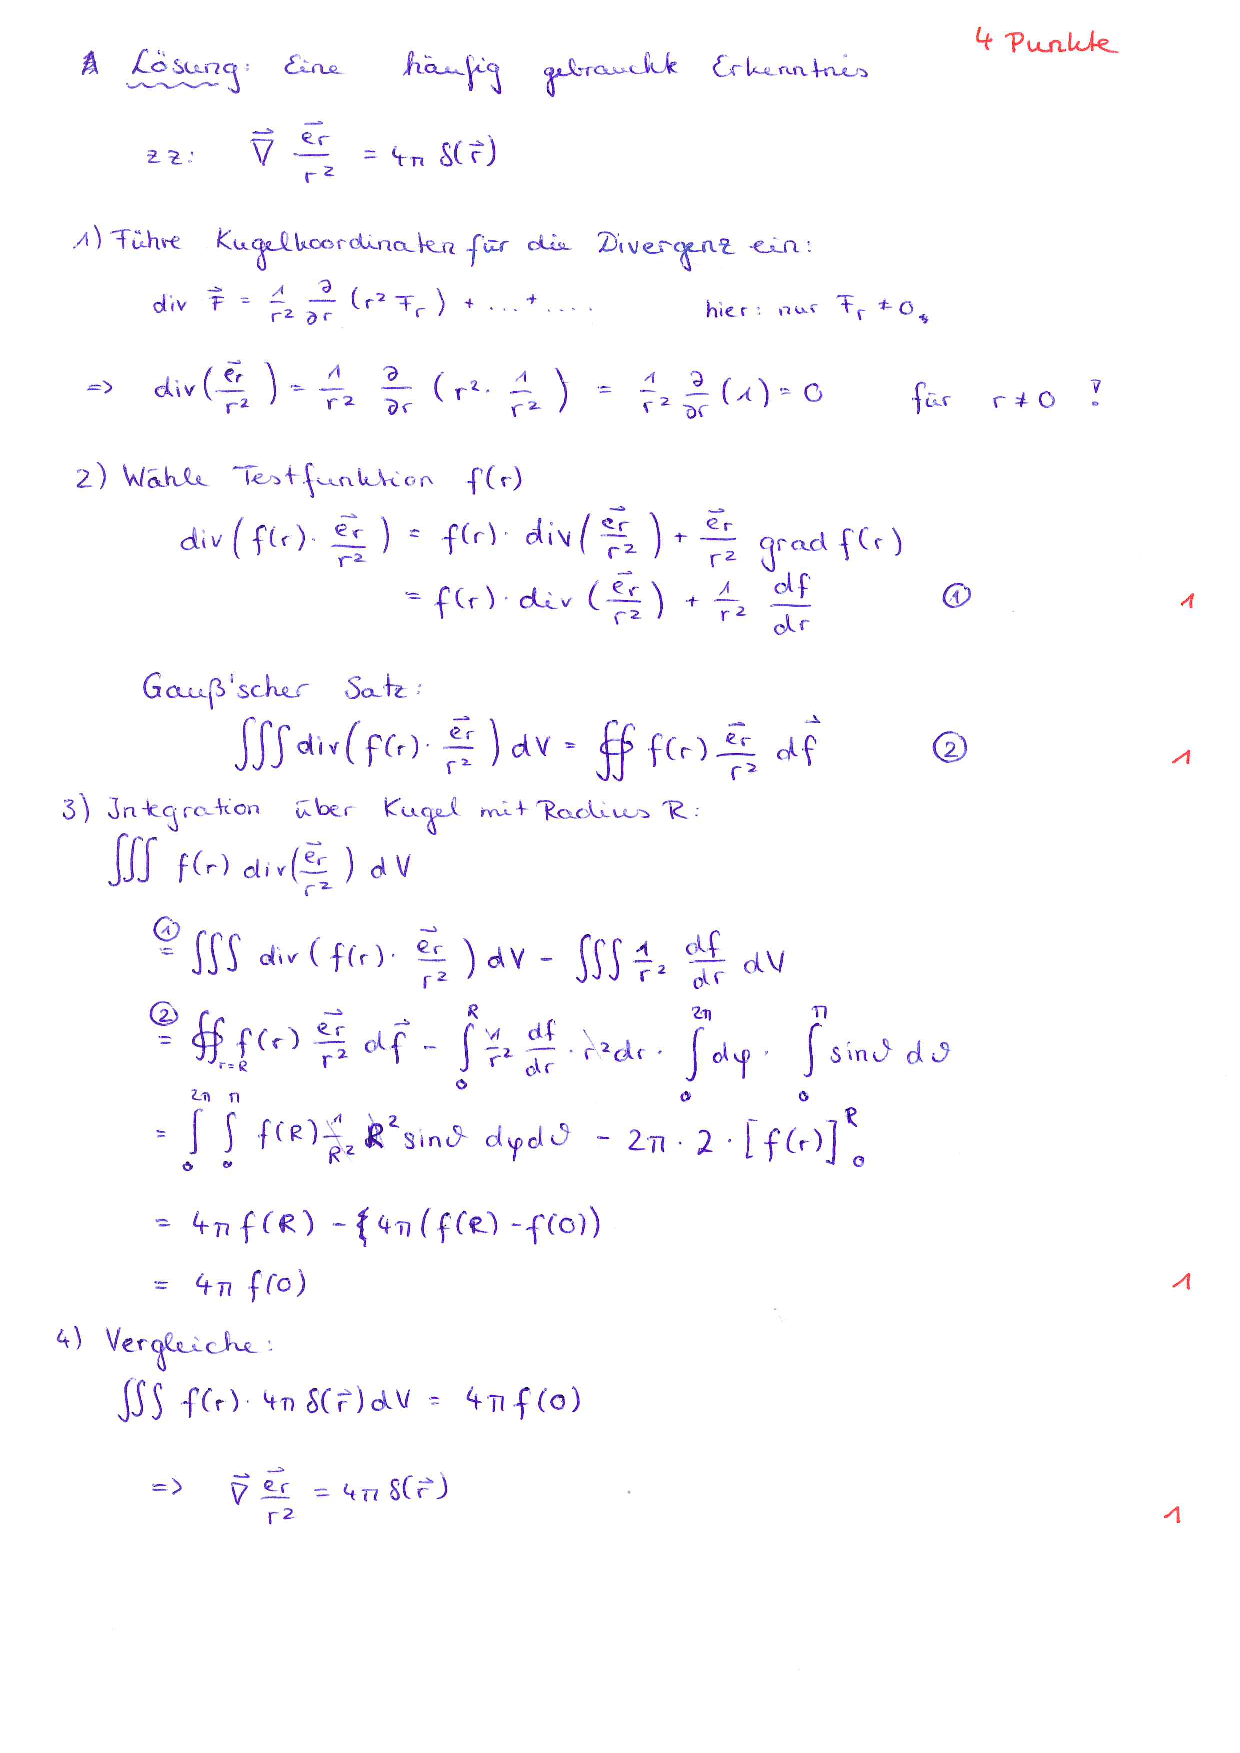
\includepdf[pages=-]{solution-delta_vi.pdf}
  \end{atiSolution}
\end{document}